\chapter{MLops}
Una tipica pipeline per un progetto di machine learning è composta da diverse fasi:
\begin{itemize}
    \item Comprensione del problema
    \item Raccolta dei dati
    \item Comprensione dei dati
    \item Preparazione dei dati
    \item Modellazione
    \item Valutazione
    \item Deployment
\end{itemize}
\begin{figure}[!ht]
    \centering
    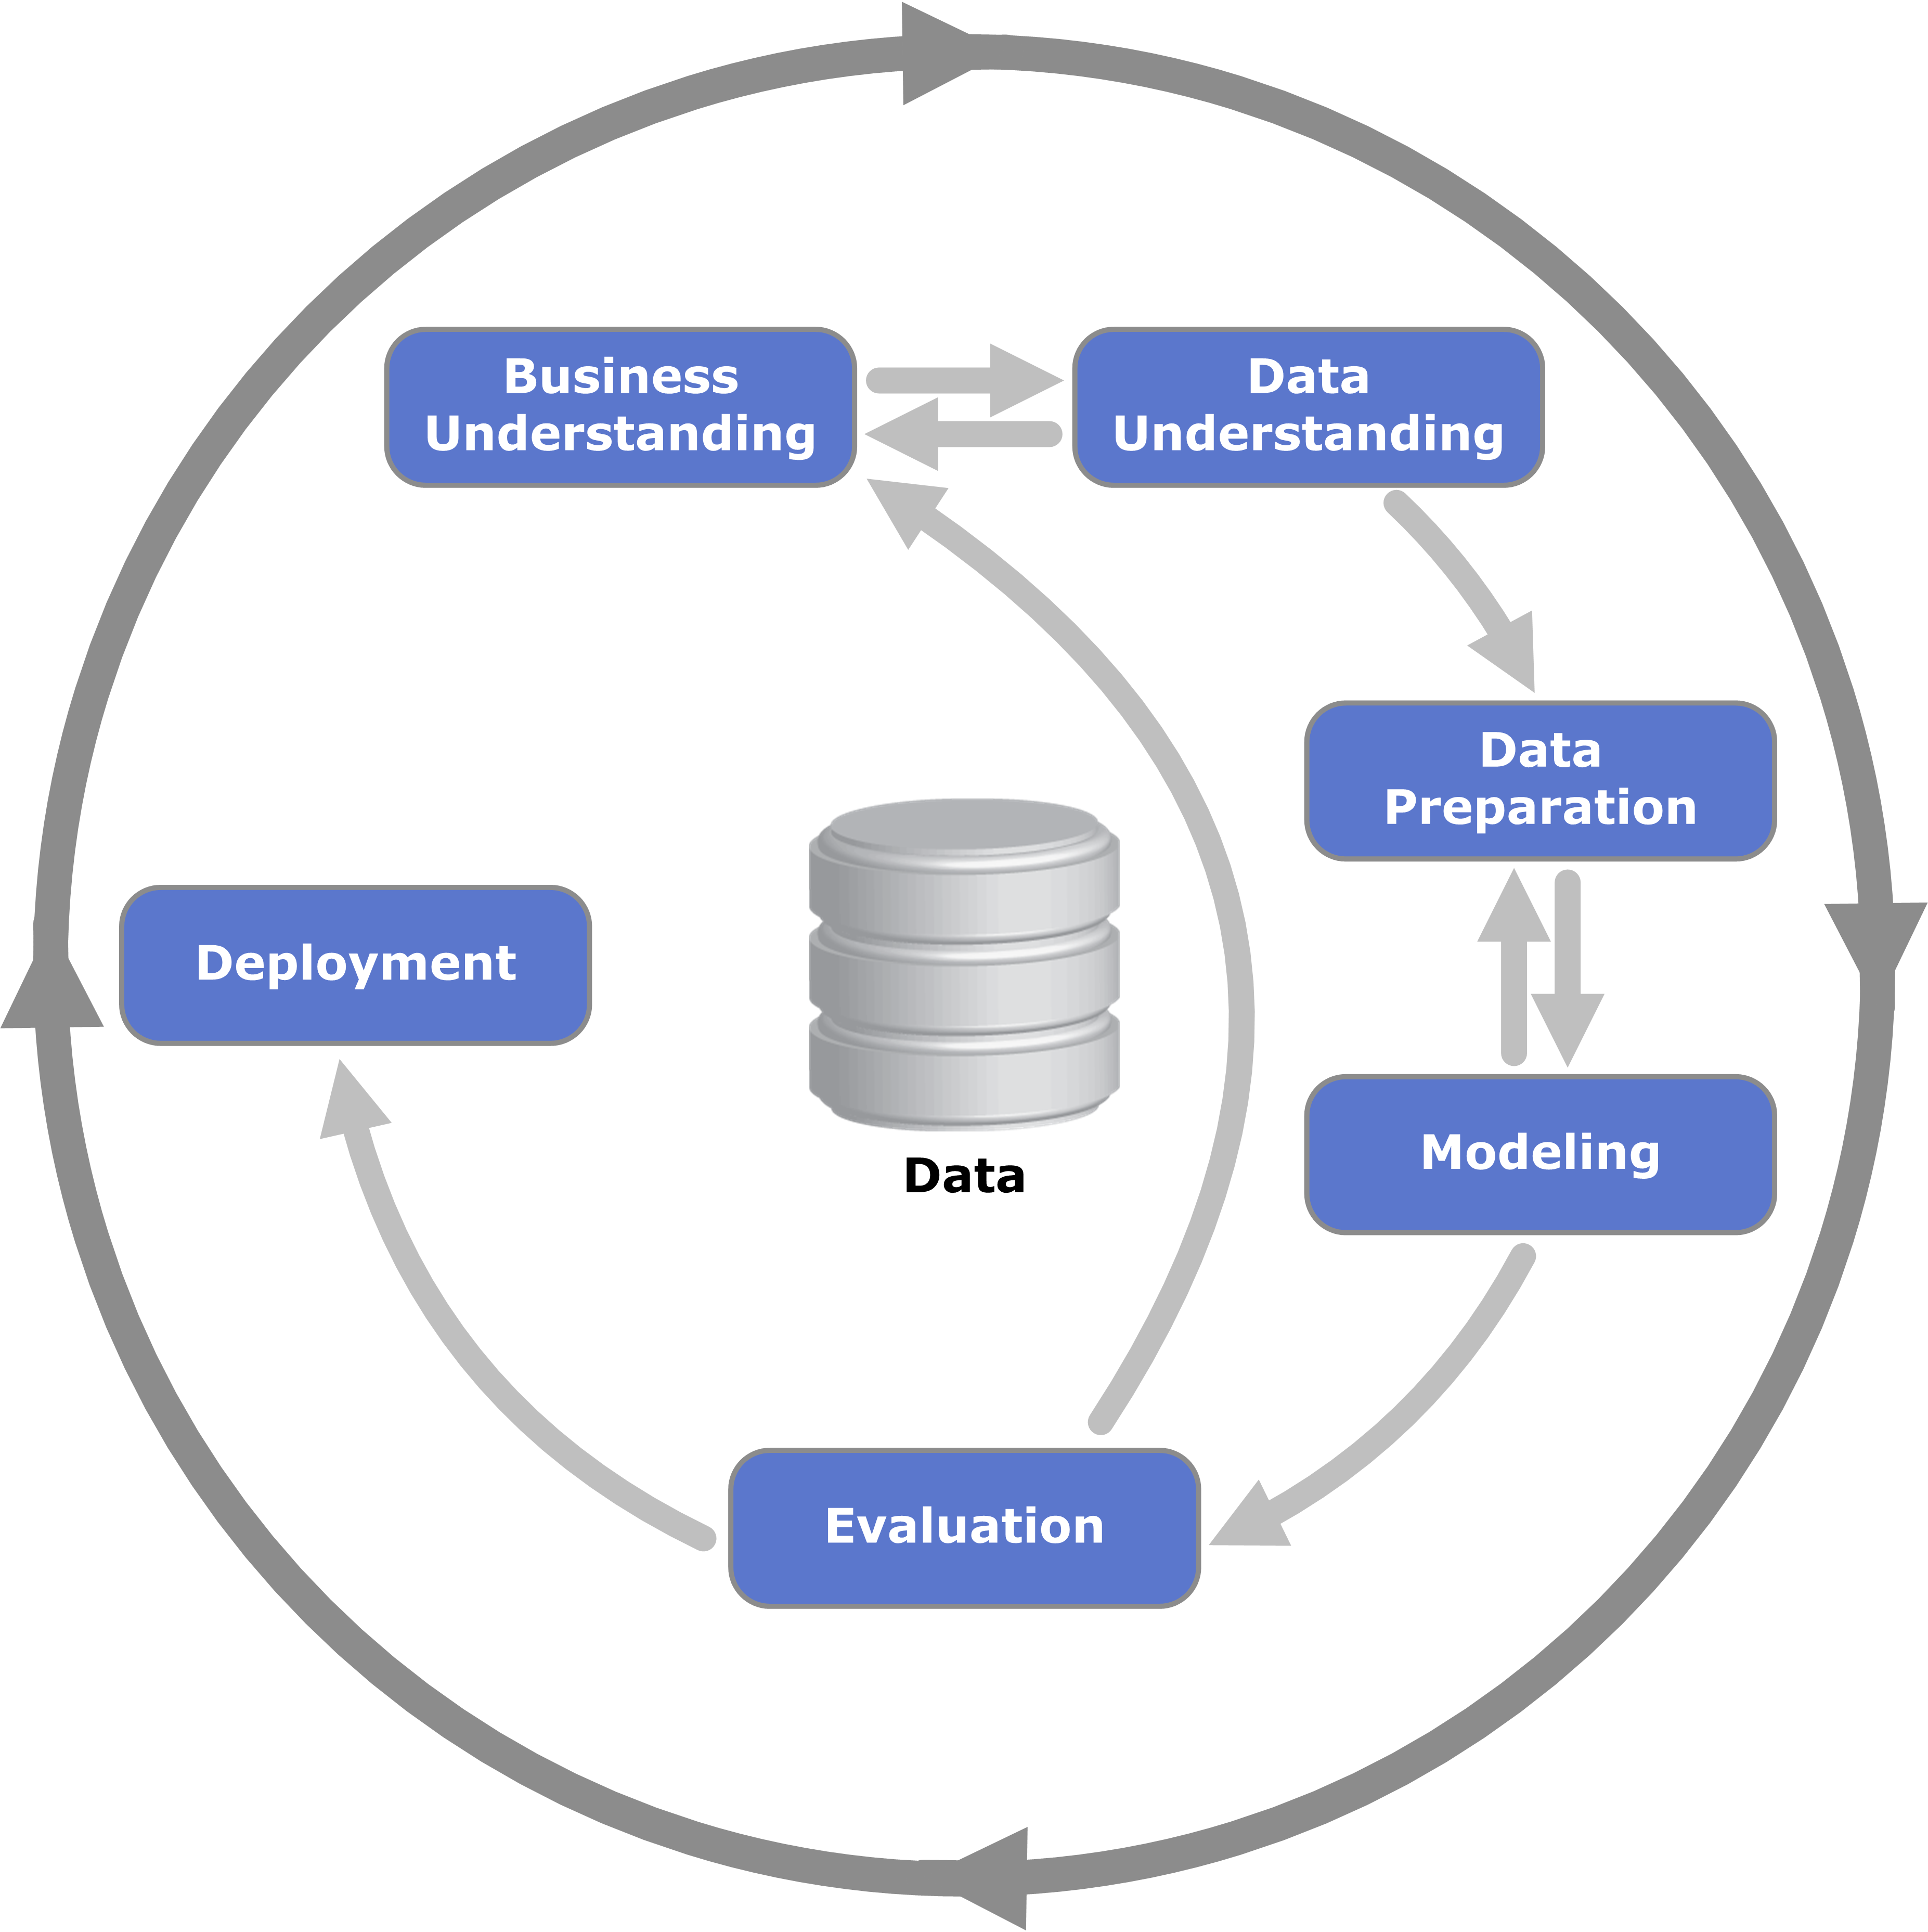
\includegraphics[width=0.5\textwidth]{./img/MLops/CRISP-DM.png}
    \caption{ML Pipeline}
    \label{fig:ml_pipeline}
\end{figure}
In questa parte del corso ci occuperemo della parte di gestione dei dati, nello
specifico analizzeremo la parte di \textbf{Data Understanding} e \textbf{Data
    Preparation}.

Avere i dati corretti è una parte fondamentale per la creazione di un modello di
che sia in grado di ottenere dei risultati corretti.
\begin{center}
    \textit{Garbage in, garbage out}
\end{center}
I dati di training e testing devono derivare dai dati reali che verranno raccolti
in fase di production.
\section{Pipeline}
Una volta ottenuti i dati reali dovremo separarli in:
\begin{itemize}
    \item \textbf{Training data}: vengono utilizzati per addestrare e valutare
          il modello, sono quindi di dimensioni elevate e vengono raccolti
          attraverso diverse fonti. Spesso caratterizzati da un elevato throughput.
    \item \textbf{Serving data}: raccolti e utilizzati per fare previsioni in
          fase di production. Questa tipologia di dati è spesso caratterizzata
          da una bassa latenza.
\end{itemize}
Entrambi questi tipi di dati devono passare attraverso una fase di preparazione.
In questa fase si vogliono stabilire quali sono le informazioni principali,
quali dati sono rilevanti e quali dati sono irrilevanti. Si effettua dunque una
prima analisi. Inoltre, vengono eseguite diverse operazioni per far si che i dati
si adattino al modello che si vuole creare.

Prima di arrivare alla parte di addestramento del modello, si passa attraverso una
fase di validazione dei dati. Questa fase è necessaria in quanto i dati cambiano
o cambia il contesto.

L'obiettivo principale è quello di capire quali feature sono significative
per il modello e quali no. Questo serve per controllare in futuro se queste
feature significative sono cambiate.

Questa fase viene fatta confrontando le distribuzioni delle features ritenute
significative durante il training con la distribuzione delle stesse feature prese
dai dati raccolti in produzione.

In questo modo possiamo segnalare quando le distribuzioni cambiano e nel caso devo
adottare delle soluzioni:
\begin{itemize}
    \item Riaddestrare il modello.
    \item Avvisare l'utente che qualcosa sta cambiando.
    \item Non fare niente.
\end{itemize}
Può capitare nel tempo i le feature cambino il tipo (ad esempio si passa da int
a float), quindi, nella fase di validation, bisogna correggerli per renderli
compatibili col modello.

Per effettuare tutti i passi della pipeline servono diverse figure lavorative:
\begin{itemize}
    \item \textbf{Machine Learning Expert}
    \item \textbf{Software Engineer}
    \item \textbf{Site Reliability Engineer}: esperto che si occupa di gestire
          tutta la pipeline e di risolvere eventuali problemi.
\end{itemize}
\section{Data Acquisition}
Una delle fasi più importanti è \textbf{Data Acquisition}. In questa fase possiamo
avere diversi problemi come ad esempio l'introduzione di bias nei dati che
invalidano i risultati del modello.

In aggiunta, è obbligatorio sapere la \textbf{Data Provenance} ovvero documentare
come ho costruito il dataset di training e validation. Questo consiste nel sapere
quali sono i dati utilizzati, da dove vengono, come ho costruito il dataset. In
questo modo si risolvono eventuali problemi dovuti a risultati sballati per dati
che sono stati iniettati nel dataset.

\section{Data Understanding}
Una volta acquisiti i dati dobbiamo interpretarli, quindi dobbiamo fare \textbf{Data 
exploration}. Per prima cosa bisogna identificare quali feature sono distribuite 
discreti e quali continui. Controllare quanti valori nulli hanno le feature, 
studi di correlazioni.

L'esplorazione dei dati può essere effettuata con dei \textbf{sanity checks} ovvero dei 
controlli sull'integrità dei dati. Per esempio la latitudine è un dato che deve 
essere compreso nel range $[-90,90]$. Tra i sanity checks si controlla il bilanciamento 
delle features, ex: una feature che può assumere i valori CALDO e FREDDO, se 
il $90\%$ degli esempi è CALDO allora non è significativa la feature. In aggiunta,
risulta fondamentale controllare anche la cardinalità dei valori.
I \textbf{sanity checks} possono essere effettuati visualizzando i dati, effettuando 
query SQL o attravarso un script.

Per gestire le inconsistenze scoperte dai sanity checks posso:
\begin{itemize}
    \item eliminare l'esempio (solo quando sono pochi)
    \item tentare di correggerlo con metodi di imputazione, bisogna però stare 
    attenti perché non sempre si può fare, per esempio se tutti i dati della feature
    di tutti gli esempi sono errati allora non posso correggerlo.
\end{itemize}

Quindi nella data exploration possiamo effettuare:
\begin{itemize}
    \item analisi univariata: identificare le feature discrete e continue,
    costruire boxplots e istogrammi per identificare outliers. Si studia la dispersione 
    dei dati, si costruiscono i boxplot, qq-plot.
    \item analisi bivariata: analisi tra coppie di variabili per studiare le correlazioni.
    Si costruiscono scatterplot tra target e una qualiasi variabile (correlazione 
    target variabili), swarmplot
\end{itemize}

è opportuno visulizzare solo informazioni utili basati sulla std.

Analisi delle features per rilevare baias.

Data lifecycle analysis analizzare se il dato prodotto è sbagliato già dalla 
sua creazione.

In aggiunta dobbiamo determinare se il modello è fair

\section{Data validation}
Controllare che la distribuzione dei dati non sia cambiata durante il tempo. Ovvero 
che non variano i valori delle variabili, in questo modo se si modifica un dato 
allora dobbiamo accorgercene per poter modificare il modello di conseguenza.

Le modifiche possono essere di questo tipo:
\begin{itemize}
    \item stringhe che passano da Upper a lower.
    \item variabili che cambiano di semantica, ex: numero di giorni che diventa 
    numero di ore. 
    \item scompare un attributo, diventa null.
\end{itemize}
Importante è avere un sistema di anomalia, sistemi di controllo che verificano che 
i dati non vengono cambianti, se venissero cambiati allora dobbiamo produrre un alert.
Un semplice alert può essere controllare che i dati delle feature siano già stati
visti. In aggiunta si deve avere un playbook per gestire chi deve accorgersi degli 
alert e chi deve risolverli. 